

\chapter{Testbench and Simulation}

\section{Introduction}

After writing some code and implementing some project in \verb|HLS|, it is time to explore the concept of \textit{testbench} and \textit{simulation}.\\

Testbench and simulation are techniques in order to validate our \verb|HLS| desing. We can validate 2 things using these concpets:

\begin{itemize}

\item functional features such as the outputs: make sure we have the correct output for some given input

\item Non-functional featrures such as timing, power consumption,$\cdots$

\end{itemize}


\autoref{fig:testbench:testbench_concept} contains the concept of a testbench

\begin{figure}[h]
\centering
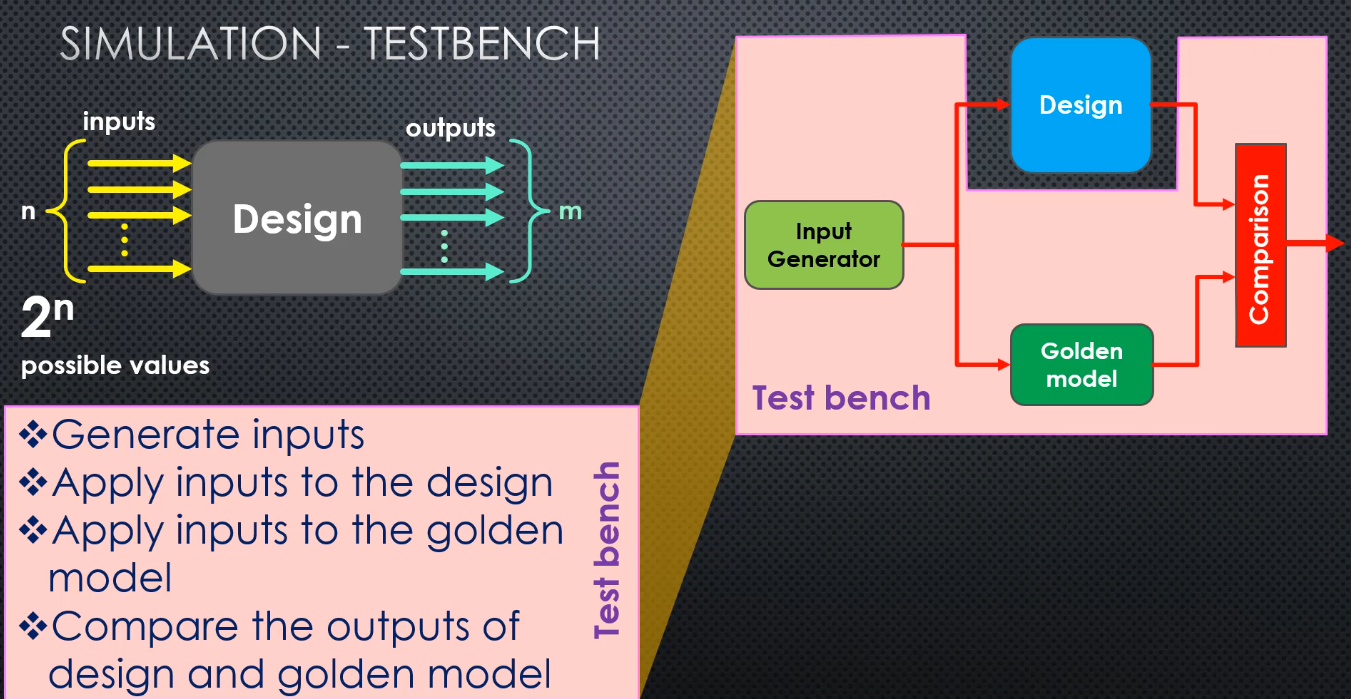
\includegraphics[scale=0.35,frame]{Figures/testbench/testbench_concept}
\caption{Testbench Concept}
\label{fig:testbench:testbench_concept}
\end{figure}

\begin{itemize}

\item Testbench is a \textit{software verification technique}, that is it relies entirely on a software approach to verify the desing

	\begin{itemize}
	\item Some other approach called \textit{emulation} rely on a software and hardware approach, in which we verify the result on the hardware target
	\end{itemize}

\item The job of a tesbench is to compare the results between our model and some state of art model using the same set of inputs, and compare the resutls to see if any differences exist

\end{itemize}

\newpage
\section{Testbench in Vitis}

Now we explore the concep using the \verb|Vitis| tool. In \verb|Vitis|, tesbench are know under the concept of \textit{C-simulation}. To understand the concept in \verb|Vitis|, we first start by recalling the classical known approach done in chapters before, that is without testbench. This approach is shown in \autoref{fig:testbench:hls_normal_flow}

\begin{figure}[h]
\centering
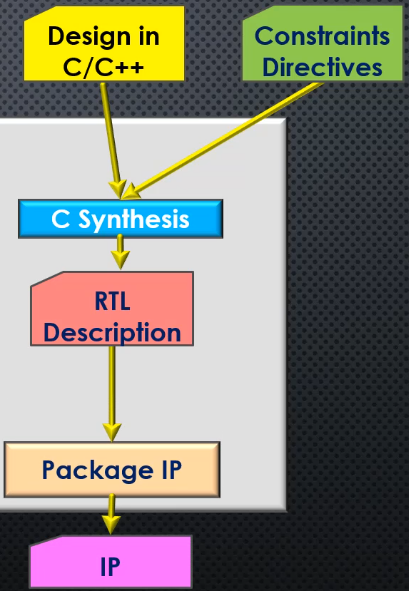
\includegraphics[scale=0.40,frame]{Figures/testbench/hls_normal_flow}
\caption{HLS Normal desing flow}
\label{fig:testbench:hls_normal_flow}
\end{figure}

\begin{itemize}

\item Using constraint file (\verb|.xdc|) and some \verb|C| code file, we generate the \verb|RTL| code (\verb|VHDL| and \verb|Verilog|) using \verb|C Synthesis| step in \verb|Vitis|.

Then in the $\mathrm{2}^\mathrm{nd}$ step, we generate the \verb|IP| so we can use it in \verb|Vivado| and generate the bitstream file to program the FPGA board.

\end{itemize}

Now to start the \textit{simulation flow}, we need 2 things: 

\begin{itemize}

\item testbench file

\item the \verb|C| files which contains the desing

\end{itemize}

\newpage
In simulation, constraint files are not needed. Using only the testbench and design \verb|C| files, we can perform \verb|C Simulation|, to correct all functional errors if any exist, and then \verb|C Sysnthesis| can be redone again to generate the \verb|RTL| code, as shown in \autoref{fig:testbench:hls_simulation}

\begin{figure}[h]
\centering
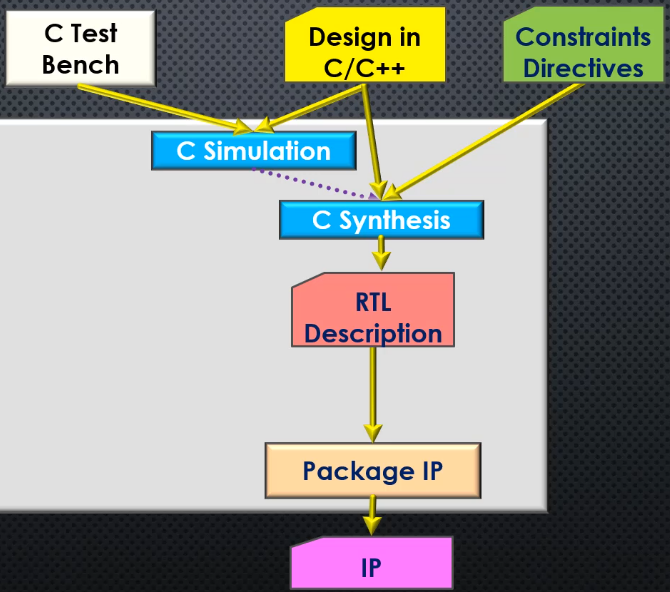
\includegraphics[scale=0.40,frame]{Figures/testbench/hls_simulation}
\caption{HLS Simulation using testbench and desing files}
\label{fig:testbench:hls_simulation}
\end{figure}


The \textit{regenerate RTL code} can also be verified, by a process called \tbi{C- RTL cosimulation}. In this process, \verb|HLS| \textit{re-uses} the testbench, and apply it on the re-gerenrate \verb|RTL|. We can check timing as well as the functinanlity in cycle accurate debug environment. 

After checking the regerenated \verb|RTL| files, the hardware \verb|IP| can be regenerate again. These steps are shown in \autoref{fig:testbench:rtl_rechecking}.


\begin{figure}[h]
\centering
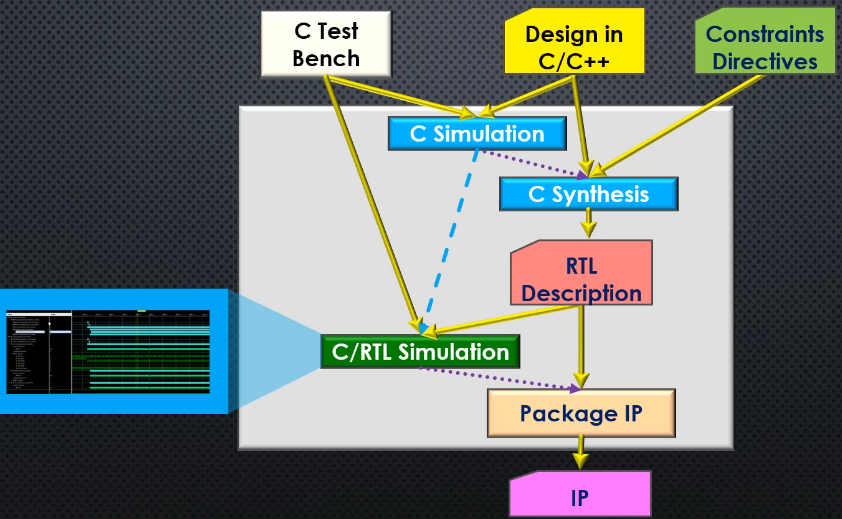
\includegraphics[scale=0.40,frame]{Figures/testbench/rtl_rechecking}
\caption{Rechecking the re-gerenated RTL code}
\label{fig:testbench:rtl_rechecking}
\end{figure}



